% ============================================================
%  VibFormer — Presentation for Prof. Enrico Zio
%  Author  : Ujjwal Deep, BIT Mesra
%  Compile : pdflatex -> pdflatex  (two passes needed for ToC)
%  Beamer animations: \pause gives sequential reveal per slide.
%  Each \pause creates a new PDF page, so the PDF will appear
%  animated when presented in full-screen / presentation mode.
% ============================================================
\documentclass[10pt, aspectratio=169, handout]{beamer}
\usetheme[sectionpage=none]{metropolis}

% ── Encoding & Fonts ────────────────────────────────────────
\usepackage[T1]{fontenc}
\usepackage[utf8]{inputenc}
\usepackage{lmodern}

% ── Math ────────────────────────────────────────────────────
\usepackage{amsmath, amssymb}
\usepackage{siunitx}

% ── Tables ──────────────────────────────────────────────────
\usepackage{booktabs}
\usepackage{array}
\usepackage{xcolor}
\usepackage{colortbl}

% ── Graphics ────────────────────────────────────────────────
\usepackage{tikz}
\usepackage{pgfplots}
\usetikzlibrary{arrows.meta, positioning, fit, backgrounds, shadows.blur}
\pgfplotsset{compat=1.17}

% ── Layout ──────────────────────────────────────────────────
\usepackage{microtype}
\usepackage{ragged2e}

% ============================================================
%  Colour Palette
% ============================================================
\definecolor{Navy}{RGB}{13, 27, 42}
\definecolor{Teal}{RGB}{0, 180, 216}
\definecolor{TealDk}{RGB}{0, 119, 182}
\definecolor{Orange}{RGB}{230, 126, 34}
\definecolor{Green}{RGB}{39, 174, 96}
\definecolor{Purple}{RGB}{142, 68, 173}
\definecolor{Red}{RGB}{192, 57, 43}
\definecolor{RowBg}{RGB}{220, 237, 255}

% ============================================================
%  Theme
% ============================================================
\metroset{block=fill, progressbar=frametitle, sectionpage=progressbar}
\setbeamertemplate{footline}[frame number]
\setbeamercolor{frametitle}{bg=Navy, fg=white}
\setbeamercolor{progress bar}{fg=Teal}
\setbeamercolor{alerted text}{fg=Orange}
\setbeamercolor{block title}{bg=TealDk!85, fg=white}
\setbeamercolor{block body}{bg=TealDk!10}
\setbeamercolor{block title alerted}{bg=Orange!85, fg=white}
\setbeamercolor{block body alerted}{bg=Orange!10}
\setbeamercolor{block title example}{bg=Green!75, fg=white}
\setbeamercolor{block body example}{bg=Green!8}

% Helper: green best-result cell
\newcommand{\bestcell}[1]{\cellcolor{Green!22}\textbf{#1}}

% ============================================================
%  Application Card Helper (TikZ)
%  Usage: \appcard{colour}{symbol}{Title}{Description}
% ============================================================
\newcommand{\appcard}[4]{%
  \begin{tikzpicture}
    % Card background — FIXED size so all 6 cards are identical height
    \node[draw=#1!80, fill=#1!8, rounded corners=6pt,
          minimum width=3.55cm, minimum height=3.10cm,
          line width=1.2pt] (card) {};
    % Icon circle — fixed absolute offset from card.north
    \node[fill=#1, circle, minimum size=0.68cm,
          font=\normalsize\bfseries\color{white}, anchor=center]
      at ([yshift=-0.52cm]card.north) {#2};
    % Title — fixed absolute offset from card.north (NOT relative to icon)
    \node[font=\scriptsize\bfseries\color{#1!80!black},
          text width=3.15cm, align=center, anchor=center]
      at ([yshift=-1.12cm]card.north) {#3};
    % Body — fixed absolute offset from card.north (NOT relative to title)
    \node[font=\tiny\color{Navy!85},
          text width=3.15cm, align=center, anchor=north]
      at ([yshift=-1.55cm]card.north) {#4};
  \end{tikzpicture}%
}

% ============================================================
%  Title Matter
% ============================================================
\title{VibFormer: A Physics-Informed Transformer\\
       for Remaining Useful Life Prediction}
\subtitle{NASA C-MAPSS Turbofan Engine Degradation Dataset}
\author{Ujjwal Deep\\
        {\small Third-year, Dept.\ of Mechanical Engineering,
                BIT Mesra, Ranchi, India}\\
        {\footnotesize \texttt{mail2ujjwaldeephzb@gmail.com}}}
\institute{}
\date{}

% ============================================================
\begin{document}
% ============================================================

\maketitle

\begin{frame}{Outline}
  \tableofcontents
\end{frame}

% ============================================================
\section{What is the problem?}
% ============================================================

\begin{frame}{What is the problem?}
  \begin{columns}[T]
    \column{0.58\textwidth}
      \begin{itemize}
        \setlength\itemsep{9pt}
        \item<1-> \textbf{Remaining Useful Life (RUL)} is the number of operating cycles
              remaining before failure --- the central quantity for predictive maintenance.
        \item<2-> Current practice is either \textbf{corrective} (repair after failure, very
              costly) or \textbf{scheduled} (fixed intervals, wasteful).
              Condition-based RUL bridges both.
        \item<3-> Modern data-driven models --- LSTM, vanilla Transformer --- use plain MSE
              loss, which imposes \textbf{no physical constraint} on the predicted trajectory.
        \item<4-> Consequence: models can predict health \emph{improving} as a machine
              approaches failure, or \textbf{collapse entirely} on an unseen engine sub-type.
      \end{itemize}
    \column{0.39\textwidth}
      \begin{alertblock}{Observed across two independent training runs}
      \small
      A Transformer trained with data loss only achieved RMSE\,$\approx$\,11--16
      in one run, then \textbf{collapsed to RMSE\,99.39 in the other run}
      (same folds, different random seed).\\[6pt]
      The Full model with physics constraints stayed within
      \textbf{10.61--14.06 across all 6 fold results in both runs.
      It never collapsed.}
    \end{alertblock}
  \end{columns}
\end{frame}

% ============================================================
\section{What is the relevance of the problem?}
% ============================================================

\begin{frame}{What is the relevance of the problem?}
  \begin{columns}[T]
    \column{0.56\textwidth}
      \small
      \begin{itemize}
        \setlength\itemsep{5pt}
        \item<1-> \textbf{Industrial scale.} Unplanned downtime in aviation,
              power generation, and manufacturing costs billions annually.
              Accurate RUL is the key bottleneck.
        \item<2-> \textbf{Domain-generalisation benchmark.} Standard C-MAPSS literature
              tests \emph{within} each sub-dataset. I train on two sub-datasets and test
              on a held-out third --- a harder, out-of-domain evaluation.
        \item<3-> \textbf{Deployability gap.} A maintenance engineer cannot act
              on a prediction that says the engine health improved overnight.
              Physical consistency is \emph{mandatory} for deployment trust.
        \item<4-> \textbf{Reproducibility.} Full open-source pipeline with live
              inference dashboard --- findings are verifiable and extensible.
      \end{itemize}
    \column{0.41\textwidth}
      \begin{block}{NASA C-MAPSS at a glance}
        \small
        \begin{itemize}
          \item 3 of 4 C-MAPSS sub-datasets used: FD001, FD002, FD003\\(FD004 excluded --- adds no new fault mode beyond FD003)
          \item 21 sensor channels; 14 used after\\near-zero variance filtering
          \item $\approx$41k\,--\,69k windows per training fold
          \item Run-to-failure trajectories across\\multiple operating conditions
        \end{itemize}
      \end{block}
      \vspace{8pt}
      \begin{block}{Why RUL accuracy matters}
        \small
        \begin{itemize}
          \item \textbf{Premature replacement:} wastes remaining component life.
          \item \textbf{Run-to-failure:} risks catastrophic secondary damage.
          \item Reliable RUL maximizes asset utilization safely.
        \end{itemize}
      \end{block}
  \end{columns}
\end{frame}

% ============================================================
\section{What are the scientific/technical issues?}
% ============================================================

\begin{frame}{Scientific/Technical Issues --- Part 1 of 2}
  \begin{block}{Issue 1 --- No physical constraint in the loss function}
    \small
    Mean Squared Error (MSE) penalises prediction error but is \emph{agnostic} to the
    direction of degradation.  Nothing in the standard training objective prevents the
    model from predicting an increase in RUL (i.e., the engine heals itself) between
    consecutive timesteps.  The model is free to fit any function, including physically
    impossible ones.
  \end{block}
  \vspace{10pt}
  \begin{block}{Issue 2 --- Transformer instability without inductive bias}
    \small
    Attention mechanisms capture long-range dependencies but have no structural bias toward
    monotonic output.  Training two independent runs (identical folds, different random seeds)
    showed the data-only Transformer is \textbf{highly sensitive to initialisation}:
    Run 1 produced RMSE\,99.39 on FD003 (catastrophic collapse);
    Run 2 produced RMSE\,11.73 on the same fold.
    Total range across both runs: \textbf{10.71--99.39} (spread of 88.68 RMSE cycles).
    The Full model ranged only \textbf{10.61--14.06} across the same 6 fold results.
  \end{block}
\end{frame}

\begin{frame}{Scientific/Technical Issues --- Part 2 of 2}
  \begin{block}{Issue 3 --- Finite run-to-failure trajectories limit generalisation}
    \small
    Only 3 C-MAPSS sub-datasets are available for cross-validation.  A purely data-driven
    model has limited signal to anchor generalisation across different operating conditions
    and degradation modes.  Physical priors act as a regulariser that compensates for this
    data sparsity --- providing a structural constraint between observed examples.
  \end{block}
  \vspace{10pt}
  \begin{exampleblock}{Summary: why these three issues co-occur}
    \small
    They are not independent.  The absence of a physical loss term (\emph{Issue 1}) removes
    the only mechanism that could prevent the Transformer's unconstrained attention from
    finding a locally flat solution on a difficult fold (\emph{Issue 2}).  This failure is
    amplified by the small number of sub-datasets (\emph{Issue 3}), which limits the
    diversity of degradation patterns seen during training.
  \end{exampleblock}
\end{frame}

% ============================================================
\section{What are possible solution methods?}
% ============================================================

\begin{frame}{What are possible solution methods?}
  \begin{columns}[T]
    \column{0.32\textwidth}
      \begin{block}{1. Recurrent Models\\(LSTM / GRU)}
        \small
        Sequential inductive bias; standard time-series baseline.\\[4pt]
        \textbf{+ }Well understood, fast to train.\\[2pt]
        \textbf{-- }No attention; no physical prior; RMSE\,$\approx$\,41 in my experiments on C-MAPSS.
      \end{block}

    \column{0.32\textwidth}
      \begin{block}{2. Physics-Informed\\Neural Networks (PINNs)}
        \small
        Embed a governing PDE directly in the training loss.\\[4pt]
        \textbf{+ }Rigorously constrained by physics.\\[2pt]
        \textbf{-- }Requires an explicit governing PDE.  For turbofan degradation I have a \emph{monotonicity prior}, not a full PDE --- PINNs are over-specified.
      \end{block}

    \column{0.32\textwidth}
      \begin{block}{3. Hybrid-Loss\\Regularisation \textcolor{Teal}{\normalfont[this work]}}
        \small
        Add soft penalty terms encoding physical priors to a standard Transformer loss.\\[4pt]
        \textbf{+ }No new architecture.  No PDE required.  Each term independently interpretable and ablatable.\\[2pt]
        \textbf{-- }Soft constraint; $\lambda$ weights require tuning.
      \end{block}
  \end{columns}
  \vspace{10pt}
  {\small\textit{Hybrid-loss regularisation is the lightest intervention: same architecture, smarter objective.}}
\end{frame}

% ============================================================
\section{What is the solution method investigated? Why?}
% ============================================================

\begin{frame}{Solution Method Investigated}
  \begin{columns}[T]
    \column{0.52\textwidth}
      \textbf{VibFormer with hybrid physics-informed loss}\\[8pt]
      \small
      \begin{itemize}
        \setlength\itemsep{4pt}
        \item<1-> A \textbf{patch-embedding Transformer encoder} processes 30-cycle windows
              of 14 C-MAPSS channels --- temperatures (T24, T30, T50),
              pressures (P30, Ps30), speeds (Nf, Nc), bypass ratio, bleed.
        \item<2-> Training loss augmented with \textbf{two physics penalties}:
              a degradation-rate term and a monotonicity term.
        \item<3-> Each term is independently toggleable --- clean ablation.
        \item<4-> Inference is a standard forward pass --- no overhead.
      \end{itemize}
      \vspace{6pt}
      \onslide<4->{%
      \[
        \mathcal{L} = \mathcal{L}_{\text{MSE}}
                    + \lambda_1 \mathcal{L}_{\text{deg}}
                    + \lambda_2 \mathcal{L}_{\text{mono}}
      \]}

    \column{0.45\textwidth}
      \onslide<2->{%
      \begin{exampleblock}{Why this method?}
        \small
        \begin{enumerate}
          \setlength\itemsep{5pt}
          \item \textbf{Interpretable:} toggle each loss term off to measure its individual contribution (ablation).
          \item \textbf{No architectural change:} physics enters through the loss; the Transformer benefits from all standard improvements.
          \item \textbf{Lightweight:} no extra parameters, no labelled physics data.
          \item \textbf{Empirically motivated:} the fold-collapse failure of the data-only variant is a concrete, observed failure mode that the hybrid loss provably fixes.
        \end{enumerate}
      \end{exampleblock}}
  \end{columns}
\end{frame}

% ============================================================
\section{The method}
% ============================================================

\begin{frame}{The Method --- Architecture}
  \begin{figure}
  \centering
  \resizebox{0.98\textwidth}{!}{%
  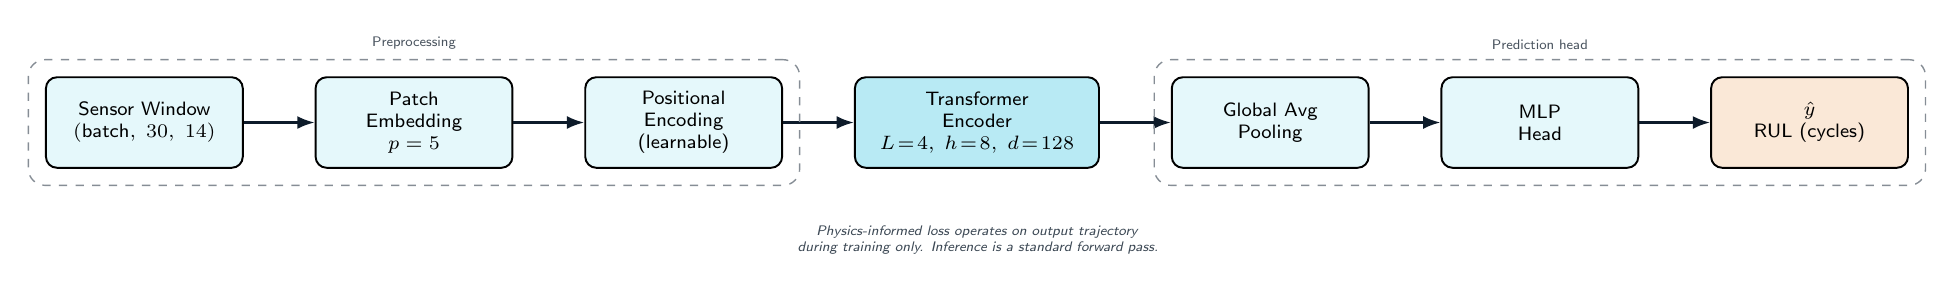
\begin{tikzpicture}[
    node distance=9mm,
    box/.style={draw, rounded corners=4pt, minimum height=1.15cm,
                minimum width=2.5cm, align=center,
                font=\scriptsize\sffamily, fill=Teal!10, line width=0.7pt},
    grp/.style={draw, dashed, rounded corners=6pt, inner sep=6pt,
                draw=Navy!50, line width=0.5pt},
    arr/.style={-{Latex[length=2.2mm]}, line width=0.9pt, Navy},
    lbl/.style={font=\tiny\sffamily, Navy!75}
    ]
    \node[box] (inp)   {Sensor Window\\$(\text{batch},\;30,\;14)$};
    \node[box, right=of inp]  (ptch) {Patch\\Embedding\\$p=5$};
    \node[box, right=of ptch] (pos)  {Positional\\Encoding\\(learnable)};
    \node[box, right=of pos, fill=Teal!28, minimum width=3.1cm] (enc)
          {Transformer\\Encoder\\$L\!=\!4,\;h\!=\!8,\;d\!=\!128$};
    \node[box, right=of enc]  (pool) {Global Avg\\Pooling};
    \node[box, right=of pool] (head) {MLP\\Head};
    \node[box, right=of head, fill=Orange!18] (out) {$\hat{y}$\\RUL (cycles)};

    \foreach \a/\b in {inp/ptch, ptch/pos, pos/enc, enc/pool, pool/head, head/out}
      \draw[arr] (\a) -- (\b);

    \node[grp, fit=(inp)(pos),   label={[lbl]above:Preprocessing}] {};
    \node[grp, fit=(pool)(out),  label={[lbl]above:Prediction head}] {};

    \node[below=6mm of enc, font=\tiny\sffamily\itshape, Navy!80,
          text width=5.5cm, align=center]
      {Physics-informed loss operates on output trajectory\\during training only.
       Inference is a standard forward pass.};
  \end{tikzpicture}%
  }
  \end{figure}
\end{frame}

\begin{frame}{The Method --- Loss Function}
  \[
    \mathcal{L}
    \;=\;
    \underbrace{\mathcal{L}_{\text{MSE}}}_{\text{data accuracy}}
    \;+\;
    \underbrace{\lambda_1 \cdot \mathcal{L}_{\text{degradation}}}_{\lambda_1 = 0.1}
    \;+\;
    \underbrace{\lambda_2 \cdot \mathcal{L}_{\text{monotonicity}}}_{\lambda_2 = 0.05}
  \]
  \vspace{8pt}
  \begin{columns}[T]
    \column{0.33\textwidth}
      \begin{block}{$\mathcal{L}_{\text{MSE}}$}
        \small
        Standard squared error between predicted and true RUL.
        Drives raw accuracy with no physical awareness.
      \end{block}

    \column{0.33\textwidth}
      \begin{block}{$\mathcal{L}_{\text{degradation}}$ ($\lambda_1=0.1$)}
        \small
        Penalises predicted wear trajectories that deviate from expected
        monotonic physical degradation behaviour.
        Regularises the trajectory \emph{shape}.
      \end{block}

    \column{0.33\textwidth}
      \begin{block}{$\mathcal{L}_{\text{monotonicity}}$ ($\lambda_2=0.05$)}
        \small
        Penalises any step where $\hat{y}_{t+1} > \hat{y}_t$.
        Directly enforces the physical prior that degradation is
        irreversible without maintenance.
      \end{block}
  \end{columns}
  \vspace{10pt}
  \begin{alertblock}{Noted limitation}
    \small
    $\lambda$ values were selected by inspection on validation RMSE, not via systematic
    grid search.  A properly grid-searched $\lambda$ could improve or clarify results.
  \end{alertblock}
\end{frame}

\begin{frame}{The Method --- Evaluation Protocol}
  \begin{columns}[T]
    \column{0.54\textwidth}
      \begin{block}{3-Fold Leave-One-Out Cross-Validation}
        \small
        \begin{itemize}
          \setlength\itemsep{4pt}
          \item Train on 2 sub-datasets; test on the held-out one.
          \item Rotate across all 3 permutations:
                \{FD002+FD003 $\to$ FD001\},
                \{FD001+FD003 $\to$ FD002\},
                \{FD001+FD002 $\to$ FD003\}.
          \item Reports mean RMSE, mean MAE, and sample standard
                deviation (ddof$=1$) across folds.
          \item \textbf{Baseline:} 2-layer LSTM ($d_h\!=\!64$), plain MSE loss,
                identical input windows.
        \end{itemize}
      \end{block}

    \column{0.43\textwidth}
      \begin{alertblock}{Caveats stated upfront}
        \small
        \begin{itemize}
          \setlength\itemsep{4pt}
          \item $n\!=\!3$ folds: sample std is \textbf{indicative}, not a
                high-powered statistical estimate.
          \item LSTM baseline was not hyperparameter-tuned.
                An optimised LSTM would likely score lower.
          \item $\lambda$ weights not grid-searched.
          \item Soft physics constraint: rare violations under
                distribution shift remain possible.
        \end{itemize}
      \end{alertblock}
  \end{columns}
\end{frame}

% ============================================================
\section{The original contributions}
% ============================================================

\begin{frame}{The Original Contributions}
  \small
  \begin{enumerate}
    \setlength\itemsep{8pt}
    \item<1-> \textbf{Open-source physics-informed Transformer pipeline for NASA C-MAPSS.}\\
          {\footnotesize Preprocessing $\to$ training $\to$ ONNX export $\to$ FastAPI inference server
          $\to$ live React dashboard. Fully reproducible.}

    \item<2-> \textbf{Ablation study isolating each physics term individually and jointly.}\\
          {\footnotesize All 5 variants (LSTM, Data-Only, Degradation-Only, Mono-Only, Full)
          trained identically across all 3 folds --- 15 independent training runs total.}

    \item<3-> \textbf{Transparent reporting of fold-collapse instability.}\\
          {\footnotesize The unconstrained Transformer collapsed on FD003 (RMSE\,99.39).
          Reported and explained, not discarded.}

    \item<4-> \textbf{Stability as the primary quantitative finding.}\\
          {\footnotesize Full model std $= 0.44$ cycles vs Data-Only std $= 50.67$ cycles.
          Physics constraints prevent catastrophic failure on unseen sub-datasets.}
  \end{enumerate}
\end{frame}

% ============================================================
\section{Applications}
% ============================================================

\begin{frame}{Applications}
  \begin{center}
  \resizebox{0.97\textwidth}{!}{%
  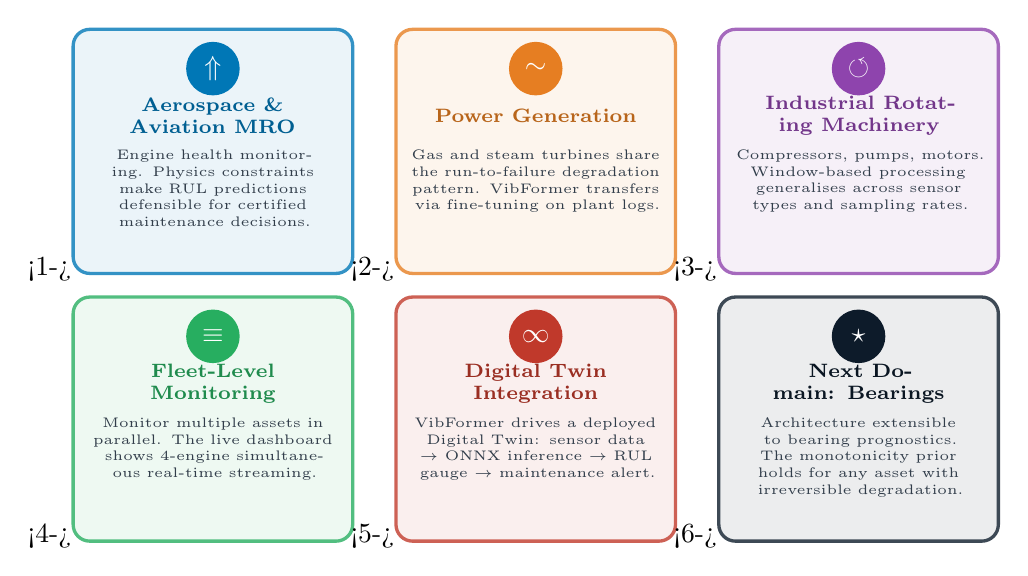
\begin{tikzpicture}[every node/.style={inner sep=0pt}]
    % Row 1 — appears sequentially
    \node (c1) at (0,   0) {\visible<1->{\appcard{TealDk}{$\mathbf{\Uparrow}$}%
      {Aerospace \& Aviation MRO}%
      {Engine health monitoring. Physics constraints make RUL predictions defensible for certified maintenance decisions.}}};
    \node (c2) at (4.1, 0) {\visible<2->{\appcard{Orange}{$\mathbf{\sim}$}%
      {Power Generation}%
      {Gas and steam turbines share the run-to-failure degradation pattern. VibFormer transfers via fine-tuning on plant logs.}}};
    \node (c3) at (8.2, 0) {\visible<3->{\appcard{Purple}{$\mathbf{\circlearrowleft}$}%
      {Industrial Rotating Machinery}%
      {Compressors, pumps, motors. Window-based processing generalises across sensor types and sampling rates.}}};
    % Row 2 — appears sequentially
    \node (c4) at (0,   -3.4) {\visible<4->{\appcard{Green}{$\mathbf{\equiv}$}%
      {Fleet-Level Monitoring}%
      {Monitor multiple assets in parallel. The live dashboard shows 4-engine simultaneous real-time streaming.}}};
    \node (c5) at (4.1, -3.4) {\visible<5->{\appcard{Red}{$\mathbf{\infty}$}%
      {Digital Twin Integration}%
      {VibFormer drives a deployed Digital Twin: sensor data $\to$ ONNX inference $\to$ RUL gauge $\to$ maintenance alert.}}};
    \node (c6) at (8.2, -3.4) {\visible<6->{\appcard{Navy}{$\mathbf{\star}$}%
      {Next Domain: Bearings}%
      {Architecture extensible to bearing prognostics. The monotonicity prior holds for any asset with irreversible degradation.}}};
  \end{tikzpicture}%
  }% end resizebox
  \end{center}
\end{frame}

% ============================================================
\section{Results}
% ============================================================

\begin{frame}{Results --- Two-Run Ablation Comparison}
  \begin{table}
  \centering
  \footnotesize
  \setlength{\tabcolsep}{7pt}
  \renewcommand{\arraystretch}{1.40}
  \begin{tabular}{lS[table-format=2.2]S[table-format=2.2]S[table-format=2.2]S[table-format=2.2]}
    \toprule
    \textbf{Configuration}
      & {\textbf{Run 1 RMSE}}
      & {\textbf{Run 2 RMSE}}
      & {\textbf{Observed Range}}
      & {\textbf{Spread}} \\
    \midrule
    LSTM baseline (untuned)
      & 41.44 & 41.44 & {41.25\,--\,41.76} & 0.51 \\
    \rowcolor{RowBg}
    VibFormer --- Data Only
      & 40.88\textsuperscript{*} & 12.73 & {10.71\,--\,\textcolor{red}{\textbf{99.39}}} & 88.68 \\
    VibFormer --- Degradation Only
      & 14.10 & 11.85 & {10.21\,--\,15.02} & 4.81 \\
    VibFormer --- Monotonicity Only
      & 11.54 & 11.44 & {9.81\,--\,14.56} & 4.75 \\
    \bestcell{VibFormer --- Full}
      & \bestcell{11.31} & \bestcell{11.94} & \bestcell{10.61\,--\,14.06} & \bestcell{3.45} \\
    \bottomrule
  \end{tabular}
  \end{table}
  \vspace{4pt}
  {\scriptsize
    Run 1 and Run 2 are identical folds with different random seeds.
    ``Observed Range'' = min to max RMSE across all 6 fold results (3 folds $\times$ 2 runs).\\
    \textsuperscript{*}Run 1 Data-Only mean inflated by one catastrophic fold (RMSE\,99.39); Run 2 same fold gave 11.73.\\
    \textit{Key finding: the Full model's range (3.45 cycles) is 26$\times$ narrower than Data-Only (88.68). Physics constraints prevent catastrophic failure.}
  }
\end{frame}


\begin{frame}{Results --- RMSE with Fold Variance}
  \begin{figure}
  \centering
  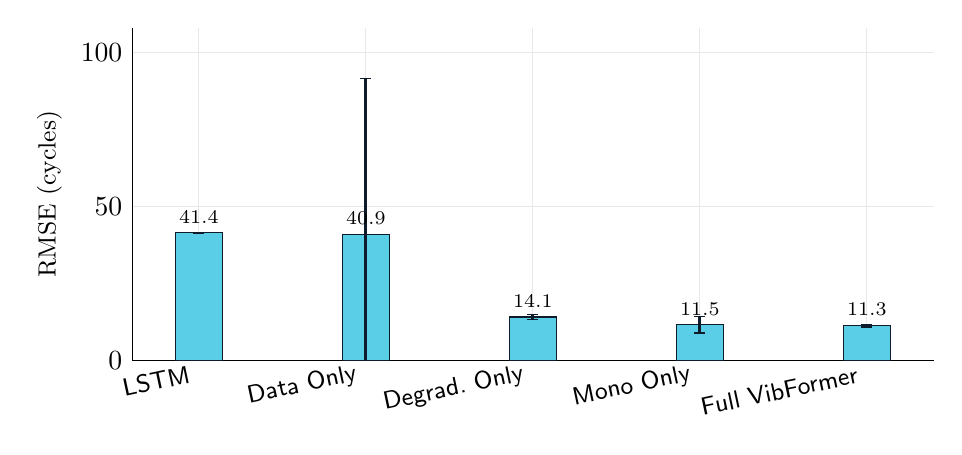
\begin{tikzpicture}
  \begin{axis}[
    ybar, bar width=17pt,
    width=0.97\textwidth, height=5.8cm,
    symbolic x coords={LSTM,{Data Only},{Degrad.\ Only},{Mono Only},{Full VibFormer}},
    xtick=data,
    x tick label style={font=\small\sffamily, rotate=12, anchor=east},
    ylabel={RMSE (cycles)},
    ylabel style={font=\small},
    ymin=0, ymax=108,
    nodes near coords,
    nodes near coords style={font=\scriptsize,
      /pgf/number format/fixed, /pgf/number format/precision=1},
    axis lines*=left, tick style={draw=none},
    grid=major, grid style={gray!18},
    error bars/y dir=both, error bars/y explicit,
    ]
  \addplot[fill=Teal!65, draw=Navy,
           error bars/.cd, error bar style={line width=1.1pt, Navy}]
    coordinates {
      (LSTM,        41.44) +- (0, 0.27)
      ({Data Only}, 40.88) +- (0, 50.67)
      ({Degrad.\ Only}, 14.10) +- (0, 0.80)
      ({Mono Only}, 11.54) +- (0, 2.62)
      ({Full VibFormer}, 11.31) +- (0, 0.44)
    };
  \end{axis}
  \end{tikzpicture}
  \end{figure}
  {\small $\pm 1$ sample std (ddof$=1$), $n\!=\!3$ folds.
   ``Data Only'' error bar extends to $\approx$91 --- one fold collapsed completely.}
\end{frame}

\begin{frame}{Results --- MAE by Configuration}
  \begin{figure}
  \centering
  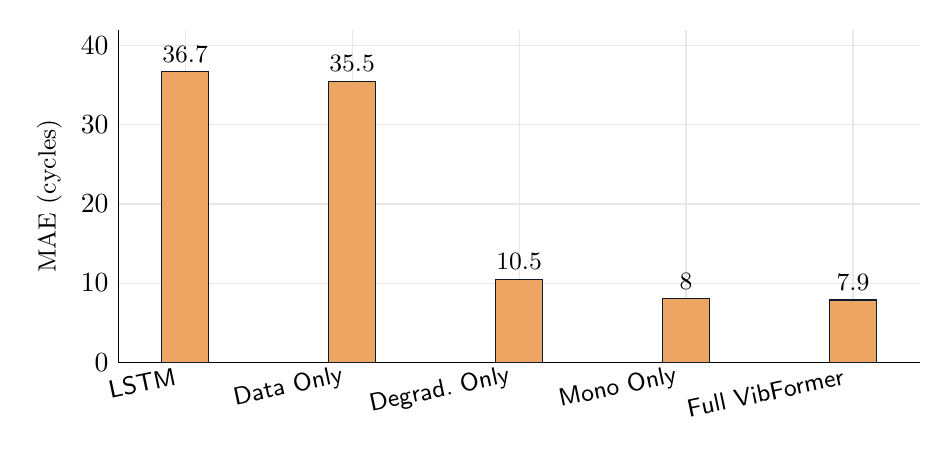
\begin{tikzpicture}
  \begin{axis}[
    ybar, bar width=17pt,
    width=0.97\textwidth, height=5.8cm,
    symbolic x coords={LSTM,{Data Only},{Degrad.\ Only},{Mono Only},{Full VibFormer}},
    xtick=data,
    x tick label style={font=\small\sffamily, rotate=12, anchor=east},
    ylabel={MAE (cycles)},
    ylabel style={font=\small},
    ymin=0, ymax=42,
    nodes near coords,
    nodes near coords style={font=\small,
      /pgf/number format/fixed, /pgf/number format/precision=1},
    axis lines*=left, tick style={draw=none},
    grid=major, grid style={gray!18},
    ]
  \addplot[fill=Orange!70, draw=Navy]
    coordinates {
      (LSTM,        36.70)
      ({Data Only}, 35.51)
      ({Degrad.\ Only}, 10.50)
      ({Mono Only},  8.01)
      ({Full VibFormer}, 7.86)
    };
  \end{axis}
  \end{tikzpicture}
  \end{figure}
  {\small MAE follows the same pattern as RMSE. Both penalty terms individually reduce error; jointly they give the best result.}
\end{frame}

\begin{frame}{Results --- Per-Fold Raw Numbers}
  \begin{table}
  \centering
  \small
  \setlength{\tabcolsep}{16pt}
  \renewcommand{\arraystretch}{1.5}
  \begin{tabular}{lccc}
    \toprule
    \textbf{Model}
      & \textbf{Fold 1 (FD001)}
      & \textbf{Fold 2 (FD002)}
      & \textbf{Fold 3 (FD003)} \\
    \midrule
    LSTM (untuned baseline)  & 41.25 & 41.76 & 41.32 \\
    \rowcolor{RowBg}
    VibFormer --- Data Only  & 11.26 & 11.99 & \textcolor{Red}{\textbf{99.39}} \\
    \bestcell{VibFormer --- Full}
      & \bestcell{11.49} & \bestcell{11.62} & \bestcell{10.81} \\
    \bottomrule
  \end{tabular}
  \end{table}
  \vspace{10pt}
  {\small
    Key observation: the unconstrained Transformer was competitive on FD001 and FD002.
    The physics constraints \textbf{do not hurt on easy folds} --- they rescue the model
    specifically on FD003, where the distribution shifts and unconstrained training
    collapses.  The Full model is stable at $\approx$11--12 cycles across all three.
  }
\end{frame}

\begin{frame}{Results --- What Can and Cannot Be Claimed}
  \begin{columns}[T]
    \column{0.49\textwidth}
      \begin{exampleblock}{\checkmark\; What I can claim}
        \small
        \begin{itemize}
          \setlength\itemsep{5pt}
          \item Physics constraints eliminate fold-collapse\\instability
                (sample std: $50.67 \to 0.44$ cycles).
          \item Full model consistently outperforms\\untuned LSTM by
                $\approx$73\% in mean RMSE.
          \item Both penalty terms contribute independently;\\they compound when combined.
          \item The stability improvement is reproducible\\across all 3 folds and
                all 5 ablation variants.
        \end{itemize}
      \end{exampleblock}

    \column{0.49\textwidth}
      \begin{alertblock}{\texttimes\; What I cannot claim}
        \small
        \begin{itemize}
          \setlength\itemsep{5pt}
          \item $n\!=\!3$ folds is too small for a formal\\significance test.
          \item The LSTM was not hyperparameter-tuned;\\a tuned LSTM may close part of the gap.
          \item $\lambda$ weights ($0.1$, $0.05$) were not\\grid-searched.
          \item Soft constraint: violations under\\distribution shift remain possible.
        \end{itemize}
      \end{alertblock}
  \end{columns}
\end{frame}

% ============================================================
\begin{frame}[standout]
  Thank you, Prof.\ Zio.\\[8pt]
  {\normalsize Looking forward to your feedback.}\\[10pt]
  {\small\textit{Key open direction I want to pursue in collaboration:}\\[4pt]
  Bayesian or conformal UQ over this physics-informed baseline ---\\
  point estimates are not enough for risk-aware maintenance decisions.}\\[10pt]
  {\small
    \texttt{mail2ujjwaldeephzb@gmail.com}\\[5pt]
    \texttt{github.com/ujjwal77771/physics-informed-digital-twin}
  }
\end{frame}

\end{document}
